\documentclass[oribibl]{llncs}
%\documentclass{llncs}
%\documentclass[citeauthoryear]{llncs}
%\documentclass[]{pasj01}
%\documentclass[draft]{pasj01}
%\documentclass[proof]{pasj01}
%\draft
%%%%%%%%%%%%%%%%%%%%%%%%%%%%%%%%%%%%%%%%%%%%%%%%%%%%%%%%%%%%%%%%
\usepackage{graphicx}
%\usepackage{listings}
\usepackage{comment}
\usepackage{color}
\usepackage{booktabs} % For formal tables
\usepackage{bm} % For formal tables
\usepackage{amsmath, amssymb}
\newcommand{\myvec}[1]{\vec{#1}}
\newcommand{\redtext}[1]{\textcolor{red}{#1}}

\newcommand{\icarus}{Icarus}
\newcommand{\pasa}{Publications of the Astronomical Society of Australia}
\newcommand{\aap}{Astronomy \& Astrophysics}
\newcommand{\aj}{The Astronomical Journal}
\newcommand{\apj}{The Astrophysical Journal}
\newcommand{\apjl}{The Astrophysical Journal Letters}
\newcommand{\mnras}{Monthly Notices of the Royal Astronomical Society}
\newcommand{\nat}{Nature}
\newcommand{\pasj}{Publications of the Astronomical Society of Japan}

%%%%%%%%%%%%%%%%%%%%%%%%%%%%%%%%%%%%%%%%%%%%%%%%%%%%%%%%%%%%%%%%

\begin{document}

\title{Global Simulation of Planetary Rings on Sunway TaihuLight}

\author{Masaki Iwasawa \inst{1} \and Long Wang \inst{1, 2} \and Keigo
  Nitadori \inst{1} \and Daisuke Namekata \inst{1} \and Takayuki
  Muranushi \inst{1} \and Miyuki Tsubouchi \inst{1} \and Junichiro
  Makino \inst{1, 3, 4} \and Zhao Liu \inst{5} \and Haohuan Fu
  \inst{6,5} \and Guangwen Yang \inst{7,6,5}}

\institute{RIKEN Advanced Institute for Computational Science \and
  Helmholtz Institut f\"{u}r Strahlen und Kernphysik \and Department
  of Planetology, Graduate School of Science, Kobe University \and
  Earth--Life Science Institute, Tokyo Institute of Technology \and
  National Supercomputing Center in Wuxi \and Ministry of Education
  Key Lab. for Earth System Modeling, and Department of Earth System
  Science, Tsinghua University \and Department of Computer Science and
  Technology, Tsinghua University}

\maketitle

\begin{abstract}

  In this paper, we report the implementation and measured performance
  of a global simulation of planetary rings on Sunway TaihuLight.  The
  basic algorithm is the Barnes-Hut tree, but we have made a number of
  changes to achieve good performance for extremely large simulations
  on machines with an extremely large number of cores.  The measured
  performance is around 35\% of the theoretical peak. The main
  limitation comes from the performance of the interaction calculation
  kernel itself, which is currently around 50\%.

\end{abstract}

\section{Introduction}
\label{sect:intro}

Our understanding of the structure of planetary rings has been advanced
greatly, mainly through interplanetary missions such as Voyager 1 and
2, and most recently Cassini. They have made a number of findings,
including the dynamic change of small-scale structures of the rings,
possibly through complex interactions with satellites. The primary
theoretical tool for the understanding of these findings is fluid
models, but many features require more detailed modeling, and direct
simulation of ring particles is necessary.

Most simulations of ring structures have been based on local
approximation, in which we apply the (pseudo-)periodic boundary
conditions for both the radial and angular
directions \cite{1988AJ.....95..925W}.

Rein and Latter (2013) used up to 200k particles to model the viscous
overstability in Saturn's rings using this local assumption
\cite{2013MNRAS.431..145R}. Because very long simulations are
necessary, the number of particles has been small. They used {\tt
  REBOUND} \cite{2012A&A...537A.128R}, an MPI-parallel $N$-body
simulation code. More recently, Ballouz et al. (2017)
\cite{2017AJ....153..146B} used {\tt pkdgrav}
\cite{2001PhDT........21S} for simulations with up to 500k particles.


Michikoshi and Kokubo (2017) \cite{2017ApJ...837L..13M} performed
global simulations of rings around the asteroid Chariklo, using 300M
particles. This is to our knowledge the largest simulation of rings
around planets (or asteroids).  They have used FDPS (Framework for
Developing Particle Simulator) \cite{2016PASJ...68...54I}, to
parallelize their calculation code.

Their calculation is probably the first global simulation of rings
with the physical size of the ring particles comparable to that of real
ones. They could do that with still a relatively small number of
particles (300M), since the asteroid and thus rings themselves are
small. If we want to model Saturn's rings, the necessary number of
particles would be much larger. The radius of the A ring of Saturn is
around $1.3\times 10^5$~km. The typical radius of ring particles is
6 m \cite{1985Icar...64..531Z}, and the optical depth of the ring is
around unity. Thus, we need $10^4$ particles per km$^2$ or around
$10^{12}$ particles for the radial range of 100 km. With this radial
range, we can model many of the fine features observed by Cassini
directly.

In this paper, we describe the result of our effort to perform such
extreme-scale simulations of planetary rings on Sunway TaihuLight, the
fastest machine as of Nov. 2016. Our implementation is also based on
FDPS, but we need to make a number of changes to the code and
algorithms to achieve reasonable performance. As a result, the
measured performance of our code, on 1/10 of TaihuLight (4096 nodes,
16384 processes) is around 31\% of the theoretical peak.

The rest of the paper is organized as follows. In
section~\ref{sec:TaihuLight}, we summarize the architecture of the Sunway
TaihuLight system and its SW26010 processor. In
section~\ref{sec:impl0}, we discuss the usual implementation of
$N$-body code on accelerator-based systems, and problems of such
an implementation on TaihuLight. In section~\ref{sec:impl1}, we describe
the algorithms we used on TaihuLight. In section~\ref{sec:result}, we
present the measured performance on TaihuLight. In
section~\ref{sec:discussion}, we summarize the results.



\section{Sunway TaihuLight}
\label{sec:TaihuLight}

Sunway TaihuLight consists of 40960 nodes, connected by a network
with injection bandwidth of 8 GB/s per node. Each node has one Sunway
SW26010 processor.  The processor consists of four ``core groups''
(CGs). One CG has one management processing element (MPE) and 64
computing processing elements (CPEs).  MPE and CPEs are both 64-bit
RISC processors and have almost the same architecture. Both MPE and
CPEs have instruction caches. MPE has L1 and L2 data caches, while
each CPE only has local data memory (LDM, 64 KB) and no cache
memory. Each CPE can still perform load/store operations to the main
memory, and they can also issue DMA transfers between LDM and the main
memory. The need for explicit control of data movement between LDM and
main memory makes the porting of the existing codes rather
complicated. On the other hand, the possibility of explicit control
makes performance tuning relatively straightforward.

The 64 CPEs in one CG is organized as an $8\times 8$ array. The
communication within the array is not mesh but point-to-point or
broadcast within the rows or columns. Thus, extremely low-latency
communication can be done within a CG, and barrier synchronization is
also extremely fast.

Operating system runs on the MPE, and the user program also runs on
the MPE. In order to use CPEs, the user either uses OpenACC or the Athread
library, which is a lightweight thread library designed for the SW26010
processor.

The processor runs with a clock speed of 1.45 GHz. Each CPE (and MPE) can
perform four double-precision multiply-and-add operations, in the form
of a 256-bit wide SIMD operation, in every clock cycle. Thus, the
theoretical peak performance of one processor is 3.016 Tflops, and
that of the entire machine with 40960 processors is 123.5 Pflops.
Each CG has 8 GB of DDR3 memory with theoretical peak transfer rate of
34 GB/s. The B/F ratio is 0.045, much lower than that of most modern
processors (both CPUs and GPUs), which is in the range of 0.15 to
0.25. Thus, it is critical to minimize the main memory access to
achieve good performance.

\section{$N$-body Algorithms for accelerator-based systems}
\label{sec:impl0}

As we have seen in the previous section, the SW26010 processor has a
``heterogeneous many-core'' architecture. Technically speaking, the
instruction-set architecture itself of MPE and CPE is almost the same,
but the absence of the data cache on the side of CPE makes the
programming mode completely different.

For accelerator-based machines, there have been a number of 
research investigations of 
optimized algorithms for gravitational $N$-body
simulations. Makino \cite{1991PASJ...43..621M} applied the
vectorizeation algorithm of Barnes \cite{1990JCoPh..87..161B} to
utilize the GRAPE hardware in combination with the Barnes-Hut tree
algorithm. Makino \cite{2004PASJ...56..521M} describes efficient
parallel implementation of the Barnes-Hut tree algorithm on GRAPE cluster
systems. This algorithm is then ported to GPGPUs \cite{Hamadaetal2009}
and has been used on many different systems.

In our FDPS system, the methods to use an accelerator is essentially the
same as those used for GRAPE or GPGPUs in the works described above.
In the original algorithm of Barnes and Hut, the tree structure is
used to approximate the forces from distant particles by the force
from their center of mass (or multipole expansion if higher accuracy
is necessary). To calculate the force on one particle in the original
algorithm, the tree structure is traversed to find the required level of
approximation.

In Barnes' modified algorithm, the tree is traversed not for each
particles but for groups of (nearby) particles, and a so-called
``interaction list'' is constructed. Then the calculation of forces on
particles in that group is done using this interaction list. In this
algorithm, tree traversal can be done on a slow general-purpose
processor, while the interaction calculation itself is done on a fast
accelerator.

For MPI-based parallelization, we need to distribute particles to MPI
processes. ORB (Orthogonal Recursive Bisection) has been used on many
parallel implementation of tree algorithms, but we used
``Multisection'' algorithm, in which the division of the domain in one
dimension is not limited to bisection but any positive integer. This
algorithm has the advantage that it can utilize non-powers-of-two
processors.

The following gives the overview of the steps of the parallel tree
algorithm on accelerator-based systems:


\begin{enumerate}

\item Perform the domain decomposition.
  
\item Exchange particles between processes so that particles belong to
  appropriate processes
  
\item Construct the local tree structure on each process.

\item Exchange the information of the tree structure necessary to
  construct a ``global tree'' on each process (so called local
  essential tree).
  
\item Construct the ``global'' tree from the collected information.

\item For each group of particles, construct the interaction list and
  perform the force calculation.
  
\item Integrate the orbits of particles.

\item Go back to step 1.
  
\end{enumerate}

Note that the construction of the interaction list and the force
calculation can be overlapped on accelerator-based systems. Thus, if
the general-purpose CPU side is not too slow, this algorithm works
extremely well, and can achieve very high efficiency.

However, in the case of TaihuLight, MPE is too slow, and the
construction of the interaction list cannot be hidden. Moreover,
relatively inexpensive calculations such as the construction of the
tree also become a large performance bottleneck. Thus, we need new
methods to reduce the calculation cost on the side of MPE.

On NVIDIA Tesla systems, B{\'e}dorf et al. \cite{2014hpcn.conf...54B}
solved this problem by moving all calculations to the GPU side.
However, in the case of the TaihuLight system, we estimated that because
of the very limited main memory bandwidth, just moving all
calculations to CPEs is still not enough. The expected performance was
below 10\%.

In the next section, we describe the new algorithms we implemented to
achieve good performance on TaihuLight.

\section{New algorithms}
\label{sec:impl1}

In this section, we describe algorithms we modified for simulating
a self-gravitating planetary ring on TaihuLight. What we have
implemented are:

\begin{enumerate}
\item The re-use of the interaction list over multiple timesteps to
  reduce the cost of both tree construction and tree traversal
\item The construction of the tree in cylindrical coordinates to optimize
  domain geometry
\item Coordinate rotation to reduce the migration of particles between
  processors
\item Eliminate the global all-to-all communication for the local
  essential tree exchange
\item ``semi-dynamic'' load balance between CPEs
\item manual tuning of the interaction kernel
\end{enumerate}  

In the following, we briefly describe these new methods.

\subsection{The re-use of the interaction list}
\label{subsec:list}

In the simulation of rings around planets, the timestep is chosen to
be small enough to resolve physical collisions between particles, and
thus relative positions of particles do not change so much in one
timestep. This is quite different from other gravitational many-body
simulations such as cosmological simulations, in which single particle
can move a distance comparable to the typical interparticle
distance. Thus, for ring simulations, it is possible to use the same
interaction list for a number of timesteps. This is essentially the
same as the ``bookkeeping'' method used in molecular dynamics
simulations, but we construct not just the list of particles but the
list of particles and tree nodes.

One issue when reusing the same interaction list over multiple timesteps is that the calculated force can be inaccurate. This can happen when the distance between a tree node in an interaction list and a particle in the group of particles corresponding to the list becomes smaller than the distances at which  physical collision occurs or the center-of-mass approximation breaks down for a given opening criterion of the tree $\theta$ while reusing the list.

We avoid this problem by constructing an interaction list so that it stores all the particles whose distances from any of the particles in the group are smaller than a pre-specified search radius as particles, not as tree nodes. By taking a sufficiently large search radius, we can calculate all the interactions correctly during the reuse steps. An appropriate value of it depends on the dynamical properties of a physical system simulated as well as the number of the reuse steps. In this study, we determine it by performing simulations repeatedly.

This functionality is now provided as an optional feature in our FDPS
distribution. 

\subsection{Tree and Domain structures on Cylindrical Coordinate}
\label{subsec:cylcoord}

One problem with handling a narrow ring with a general-purpose domain
decomposition algorithm is that the shape of some of the domains can
become highly irregular, resulting in an increase in communication
between processes. Figure~\ref{fig:domain_cart} shows an example. We
can see the domains near the $y$ axis are very elongated.

\begin{figure}
  \centering 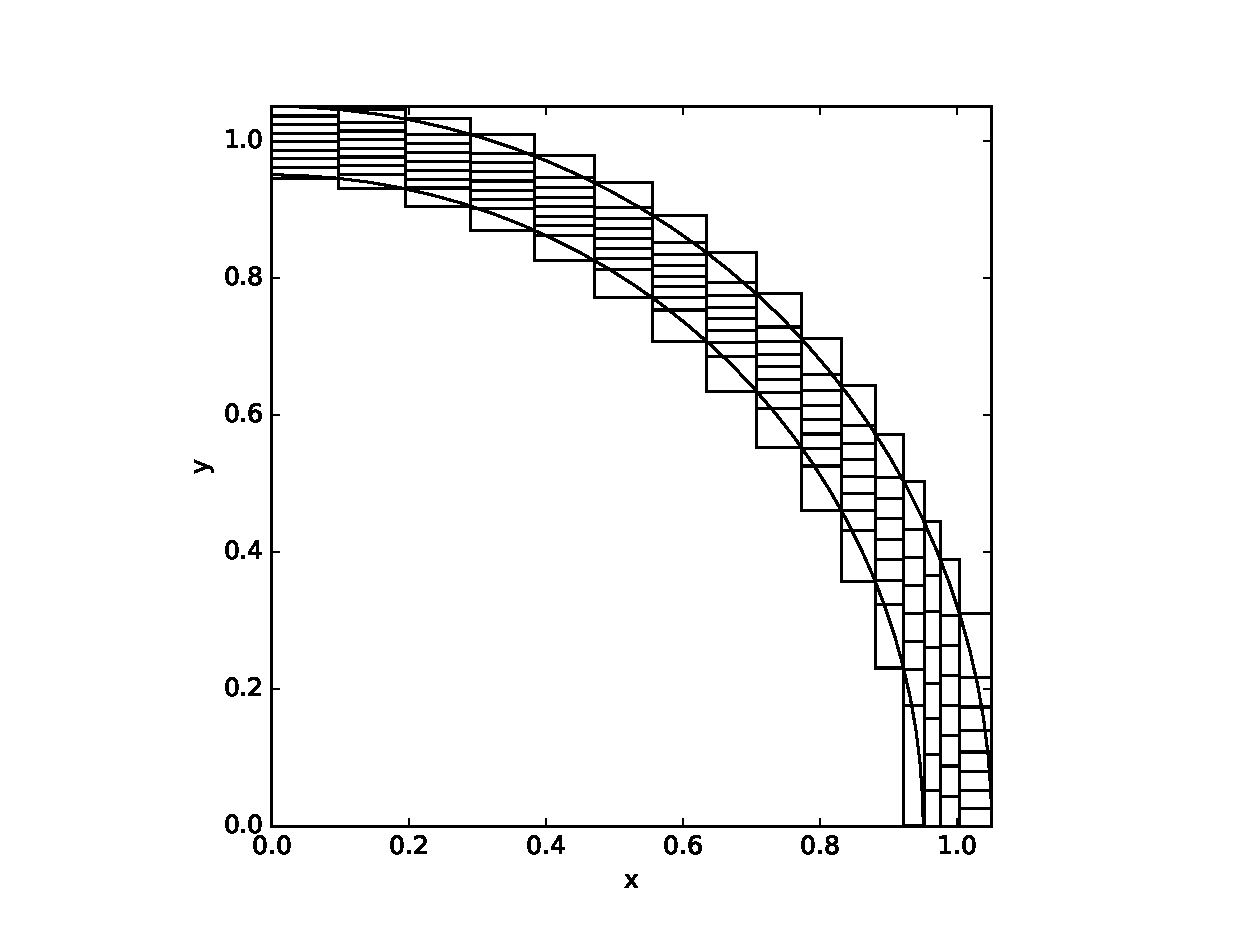
\includegraphics[width=8cm,clip]{./fig/domain_cart.eps}
  \caption{Schematic figure of domain decomposition by the multisection
    method in $x$-$y$ coordinate. Domains are divided by $16 \times 8$.}
  \label{fig:domain_cart}
\end{figure}

\begin{figure}
  \centering
    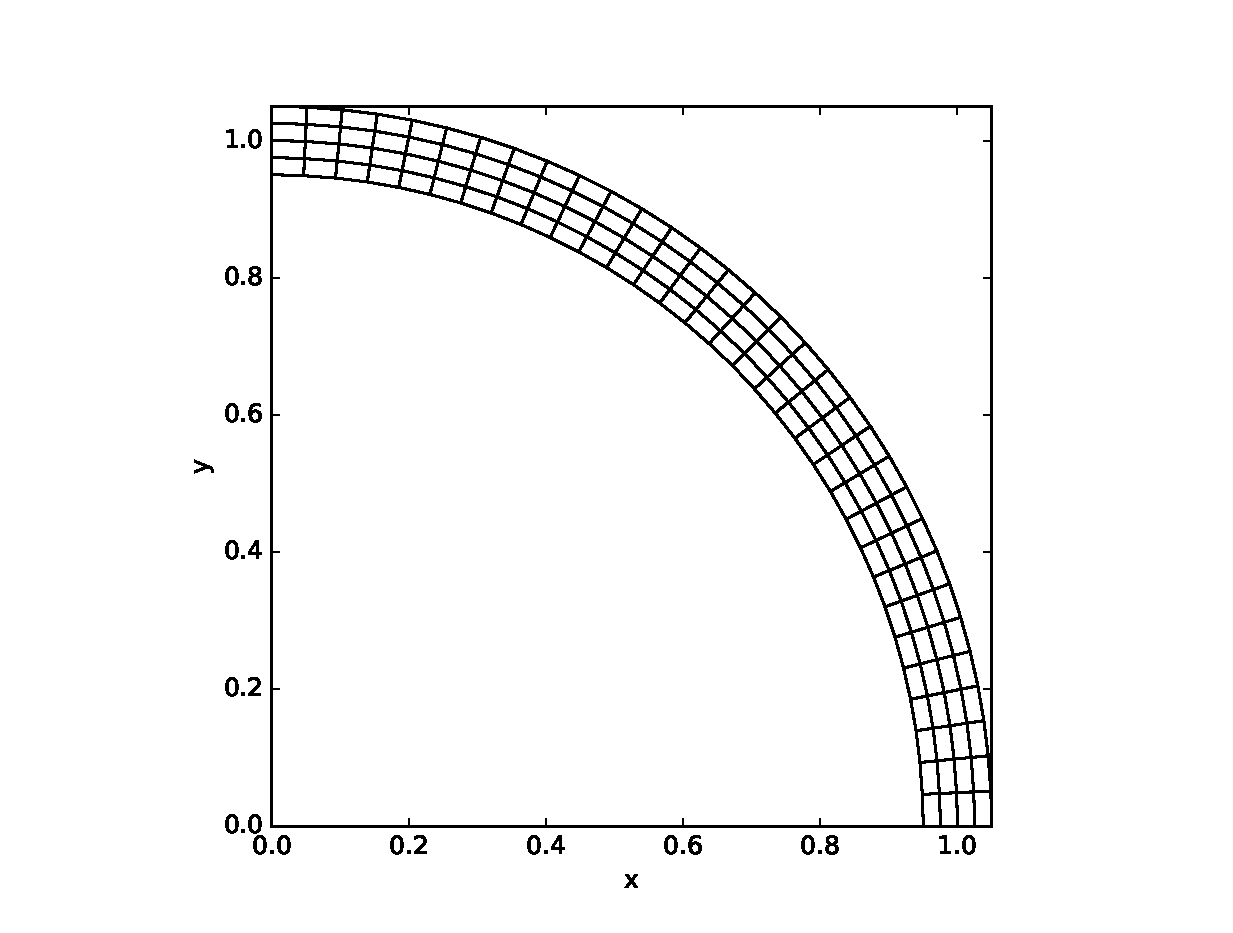
\includegraphics[width=8cm,clip]{./fig/domain_cyl.eps}
  \caption{Schematic figure of domain decomposition by the multisection
    method in cylindrical coordinate. Domains are divided by $4 \times 32$.}
  \label{fig:domain_cyl}
\end{figure}

The reason why the shapes of domains become irregular is that we are
trying to fit a circle to squares and rectangles. A natural way to
apply domain decomposition is to use polar coordinates and apply
divisions in radial and angular directions.

Conceptually the simplest approach is thus to use polar coordinate
(cylindrical in this case) for positions and velocities of particles,
and also for coordinates for constructing the tree structure. Since
the ring is narrow, the local distance $s$ in the Cartesian coordinate
$(x, y, z)$ can be approximated by that in cylindrical coordinate
($r$, $\phi$, $z$).
\begin{equation}
  \label{eq:metric}
  ds^2 = dx^2 + dy^2 + dz^2 \sim d\phi ^2 + dr^2 + dz^2,
\end{equation}
when $r \sim 1$. This means that, for domain decomposition and tree
construction and even for tree traversal, we can just use polar
coordinates, without any modification of the algorithm or program
itself. The interaction calculation is faster in Cartesian
coordinates and thus Cartesian coordinates should be used.

Figure~\ref{fig:domain_cyl} shows the domain decomposition in
cylindrical coordinates. We can see that all the domains have similar,
near-square shapes.

\subsection{Coordinate rotation}
\label{subsec:exptcl}
 
In any parallel tree algorithm, domain decomposition is done in fixed
coordinates, while particles move around. If the distribution of
particles is not changing rapidly, even if particles move, the domain
structure does not change much.

Usually, the fraction of particle that move from one domain to
another is relatively small, and the cost of this part is not
dominant, since LET exchange is more costly. However, when we use
an extremely large number of processes, and when the simulated system is
a narrow ring, at one timestep many (or all) particles can move from
one domain to another. Consider the case of using 100k processes for a
ring with the aspect ratio of 1:1000. We use a process grid of
$10\times 10,000$. Thus, if the timestep per one Kepler period is
smaller than 10,000, all particles in each domain moves to other
domain in every timestep, resulting in very high communication cost.

An obvious solution for this problem is to let the coordinates and domain
structure rotate, so that particles do not move much. If we rotate the
coordinates at the speed of Kepler rotation at the center of the ring,
particles at the center of the ring do not move much. Particles at
other radial positions do move, but at speed much smaller than
that of the Kepler rotation. Thus, communication due to Kepler
rotation can be almost eliminated.

Note that we need to (and can) apply this coordinate rotation only at
the steps in which the tree is reconstructed. Thus, the additional
calculation cost is negligible.

\subsection{Elimination of all-to-all communication}
\label{subsec:exlet}

%% \begin{figure}
%%   \centering 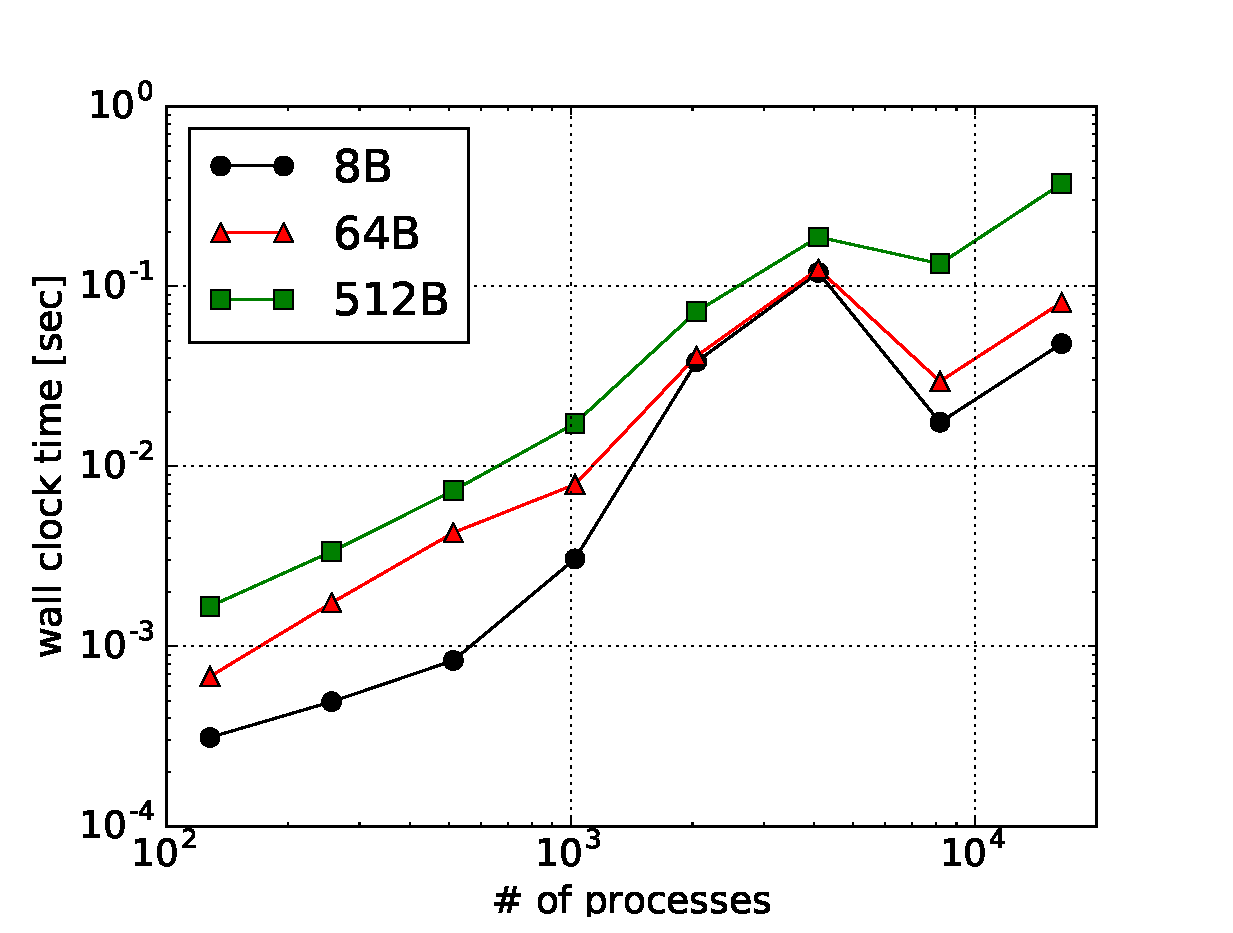
\includegraphics[width=8cm,clip]{./fig/comm_np-wtime.eps}
%%   \caption{Wall clock time for {\tt MPI\_Alltoall} against the number of processors.}
%%   \label{fig:comm_np-wtime}
%% \end{figure}

%% \begin{figure}
%%   \centering
%%   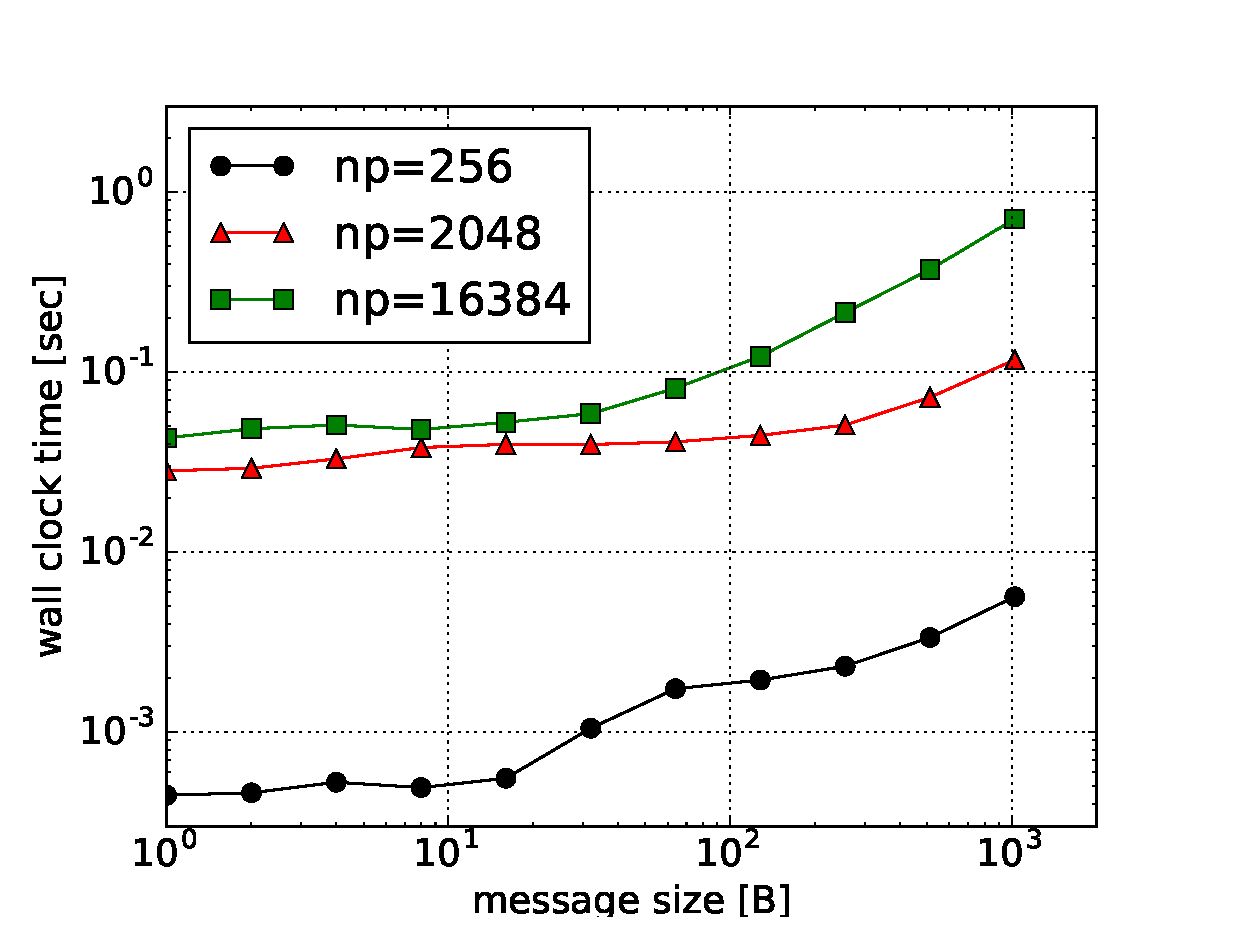
\includegraphics[width=8cm,clip]{./fig/comm_msize-wtime.eps}
%%   \caption{Wall clock time for {\tt MPI\_Alltoall} against the size of the message sent per process.}
%%   \label{fig:comm_msize-wtime}
%% \end{figure}

In FDPS, the exchange of LET (local essential tree) data is done as
follows. All processes have the information of the domain geometry of
all other processes, and thus can determine what information should be
sent. Thus, each process first constructs the necessary data for all
other processes, and then all processes send and receive information
through a single call to the {\tt MPI\_Alltoallv} function.

This implementation works fine even for 10k or more processes, but
becomes problematic on large systems like TaihuLight. Even when the
implementation of {\tt MPI\_Alltoallv} is ideal, each process
receives at least one particle (the center of mass of all particles in
one process) from each other process. Thus the total amount of LET
data proportional to the number of processes, and thus
for a large enough number of processes this part dominates.

Conceptually, we can eliminate this global communication, by
constructing the ``tree of domains'' locally and let only higher-level
information be sent to distant processes.

In the current implementation specialized to narrow rings, we
implemented a very simple two-level tree, in which the second-level
tree nodes have all processes in the radial direction. For example, if we
have a process grid of (1000, 10), where 1000 in angular and 10 in
radial direction, 10 domains in the radial direction are combined to
one tree node, resulting in 1000 second-level nodes. Only these 1000
nodes exchange their center-of-mass information. All LET information
other than these center-of-mass data of second-level nodes are sent
either to other second-level nodes (and then broadcast to
lower-level nodes) or sent directly to lower-level nodes.

In this implementation, there is still one global communication in the
angular direction, but we can use {\tt MPI\_Allgather} since only the
top-level data are sent. Thus the reduction in the communication is
quite significant.


\subsection{Load Balance between CPEs}
\label{subsec:force}

In the force calculation part, in our current implementation, each CPE
handles one interaction list at a time. MPE first prepares a large
number of interaction lists, and then CPEs process them
one-by-one. Since both the length of the interaction list and the
number of particles which share one interaction list varies by a
fairly large factor, if CPEs process the interaction lists in a fixed
order, a large load imbalance appears. In order to achieve a better
load balance between CPEs, we applied the following simple algorithm.

\begin{enumerate}
  
\item Sort the interaction lists by their length.

\item Assign the longest 64 lists on 64 CPEs.

\item For each remaining list, assign it to the the CPE with the
  shortest total calculation cost.
  
\end{enumerate}

Since the calculation time of a CPE is quite predictable, this
algorithm works very well.

We could further improve the load balance by multiple CPEs handle
one interaction list, either by dividing the list or the particles
which share the list.

\subsection{Interaction Kernel}

On CPEs, we found the compiler-generated code for the interaction
kernel, even when SIMD operations are used, does not give very good
performance. We rewrite the interaction kernel fully in assembly
language, with hand-unroll and careful manual scheduling. As a result,
we achieved more than 50\% of the theoretical peak performance for the
kernel.

\section{Measured performance}
\label{sec:result}

We have measured the performance of our code on TaihuLight with up to
4096 nodes (16384 MPI processes). In this section we present the
results.

\subsection{Initial Condition}

The ring has central radius of unity in our simulation units and its
width is 0.01. These corresponds to $10^5$ km and $10^3$ km, when we
regard this ring as Saturn's A ring.  In the weak-scaling test, the
number of particles per process is 1M, and in the strong-scaling test
the total number of particles is 2G. The mass $m$ and radius $r$ of
particles are given by:
\begin{eqnarray}
  r &\sim& 3.1 \times 10^{-5} \left( 2 {\rm G} / N \right)^{1/2}, \\ 
  m &\sim& 8.5 \times 10^{-14} \left( 2 {\rm G} / N \right)^{3/2}, 
\end{eqnarray}
where $N$ is the total number of particles. The mass of Saturn and
gravitational constant are both unity. Thus, the orbital period of
ring particles is $2\pi$.

\subsection{Interaction Model}

Ring particles interact through mutual gravity and physical inelastic
collisions. We model inelastic collisions by soft spheres with spring
and dashpot. Equation \ref{eq:interaction} gives the definition of the
particle-particle interaction.

\begin{eqnarray}
  \bm F_{ij} = \left \{
  \begin{array}{ll}
     G \frac{m_i m_j}{r_{ij}^3} \bm r_{ij} & \left(r_{ij} > r_{\rm coll} \right) \\
     \left[  G \frac{m_i m_j} {r_{\rm coll}^3} + \frac{m_j}{m_i + m_j} \left( \kappa \frac{ r_{ij} - r_{\rm coll}}{r_{ij}} + \eta \frac{\bm r_{ij} \cdot \bm v_{ij}}{r_{ij}^2} \right) \right] \bm r_{ij} & \left( r_{ij} \le r_{\rm coll} \right)
  \end{array}
  \right.
\label{eq:interaction} 
,
\end{eqnarray}
with $\bm r_{ij} = \bm r_j - \bm r_i$, $\bm v_{ij} = \bm v_j - \bm
v_i$, $r_{ij} = \| \bm r_{ij} \|$. Here, $\bm F_{ij}$ is the
acceleration of particle $i$ due to particle $j$, ${\mathbf r_{ij}}$ and
$\bm v_{ij}$ are the relative position and velocity vectors, $G$
is the gravitational constant (taken to be unity in this paper), $m_i$
is the mass of particle $i$, $r_{coll}$ is the distance at which two
particles collide, and $\eta$ and $\kappa$ are parameters which
determine the coefficient of restitution. We chose these parameters so
that the coefficient of restitution in the radial direction is 0.5, which is close to the experimental values (e.g. Hatzes et al. \cite{hatzes88:_collis}).

Particle-particle interaction consists of 9 multiplications, 8
additions, and one square root and one division
operation. The instruction set of Sunway 26010 processor does not include
fast approximation for either square root or reciprocal square
root. So we implemented fast initial guess and high-order convergence
iteration in software. The number of operations in this part is 7
multiplications, 5 additions and two integer operations. Therefore,
for particle-cell interactions the number of floating-point operations
is 31, and for particle-particle interactions, which include the
repulsive force during physical collisions, is 47. The total number of
floating-point operations is obtained by counting the number of
interactions calculated and multiplying them with these number of
floating-point operations per interaction. We ignore all operations
other than the interaction calculation, since as far as the number of
floating-point operations is concerned, the operation count for interaction
calculation is more than 99\% of the total operation count.

\subsection{Performance}

We used the opening criterion of the tree $\theta$ of 0.5. The leap
frog integrator with a timestep of $1/128$ is used. We use the same
interaction list for 64 steps.

To measure the performance, we measure the time for 64 timesteps,
including the time for diagnostics. The execution time is measured by
the MPI wallclock timer, and the operation count is from the counted
number of interactions calculated.


\begin{figure}
  \centering
    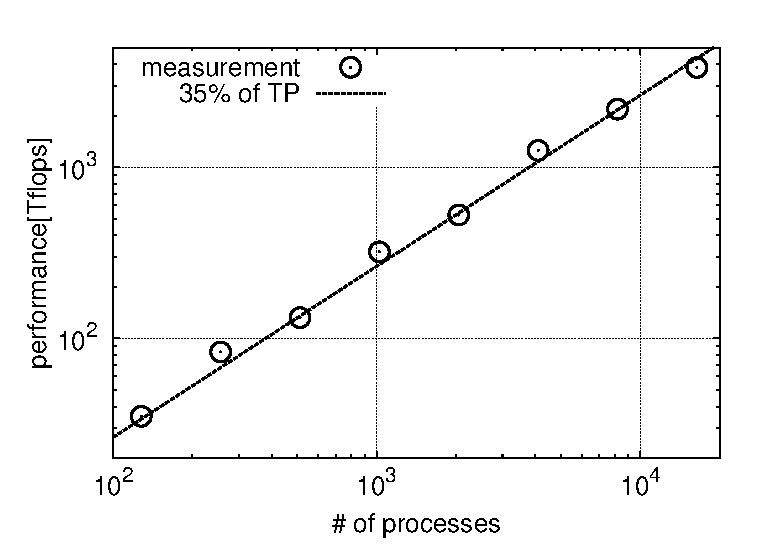
\includegraphics[width=8cm,clip]{./fig/weak_speed.eps}
  \caption{Performance in Tflops for weak-scaling test. The number
    of particles per process is 1M. Solid line indicates 35 \% of the
    theoretical peak performance of TaihuLight. Open circles indicate
    measured performance.}
  \label{fig:weakpf}
\end{figure}

\begin{figure}
  \begin{center}
    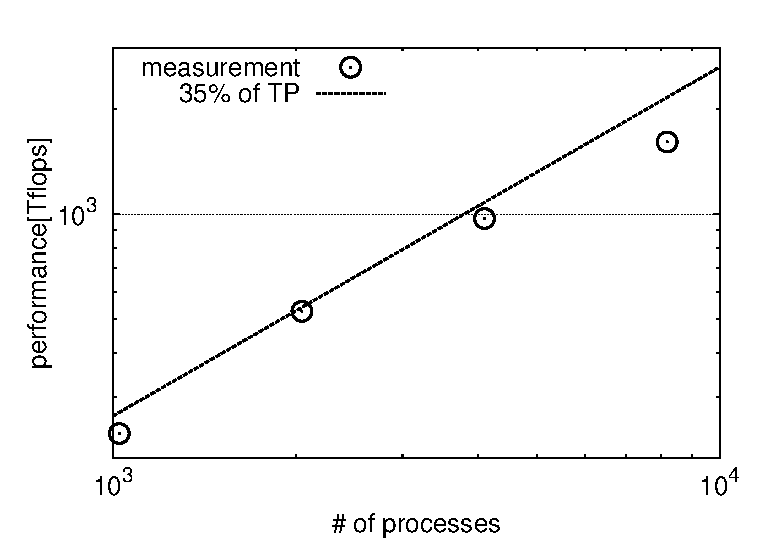
\includegraphics[width=8cm,clip]{./fig/strong_speed.eps}
  \end{center}
  \caption{Performance in teraflops for strong-scaling test. The
    number of particles per process is 2048M. Solid line indicates 
	35\% of the theoretical peak performance of TaihuLight. Open circles
    indicate measured performance.}
  \label{fig:strongpf}
\end{figure}

\begin{figure}
  \begin{center}
    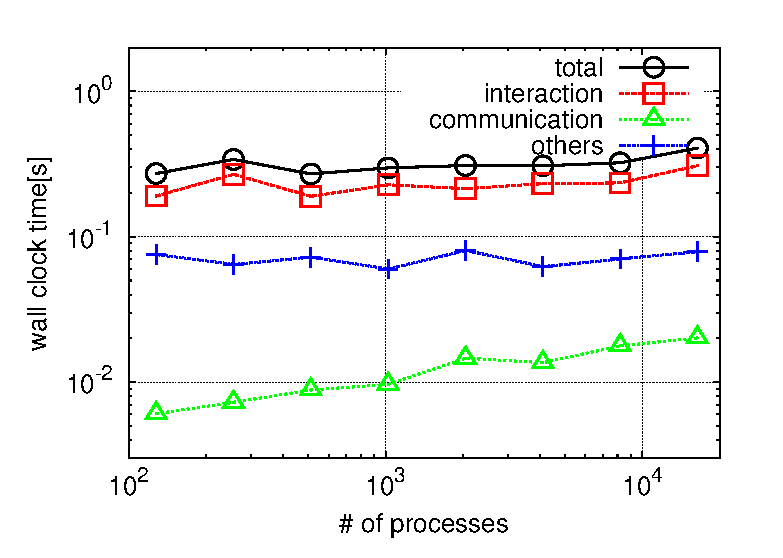
\includegraphics[width=8cm,clip]{./fig/weak.eps}
  \end{center}
  \caption{Time per timestep for weak-scaling test. }
  \label{fig:weak}
\end{figure}

\begin{figure}
  \begin{center}
    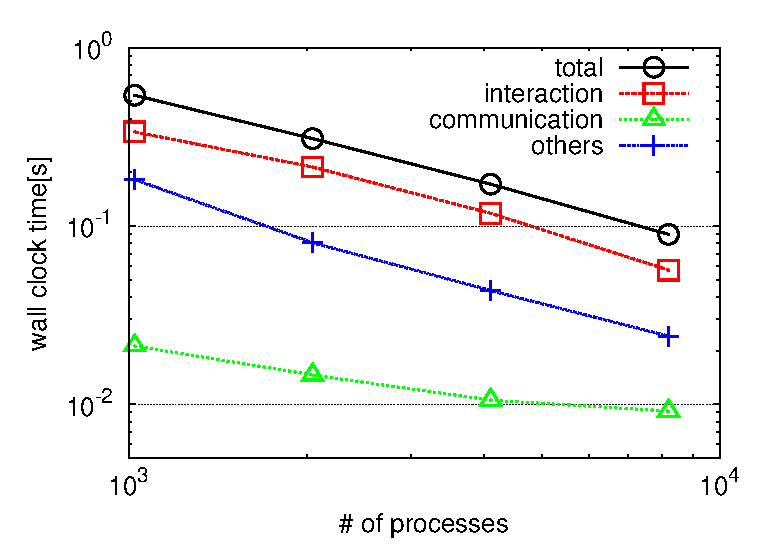
\includegraphics[width=8cm,clip]{./fig/strong.eps}
  \end{center}
  \caption{Time per timestep for strong-scaling test.}
  \label{fig:strong}
\end{figure}

Figures \ref{fig:weakpf} and \ref{fig:strongpf} show the speed in
Tflops for weak- and strong-scaling runs.  Weak-scaling result is almost
ideal. Our code runs at around 35\% of the theoretical peak
performance of TaihuLight.


Figures \ref{fig:weak} and \ref{fig:strong} show the breakdown of the
time per timestep. We can see that even for 16K processes the time for
communication is less than 10\% of the total time.


Table~\ref{tab:break_down} shows the detailed breakdown of the
calculation time for the case of a weak-scaling run with 8192 processes.
The terms for which the speedup factor is 64 are performed only once
per 64 steps. We can see that the dominant terms apart from the
interaction calculation are ``Local Tree update'', ``Global Tree
construction'', ``Global Tree update'' and ``Interaction list
construction''.  The two ``update'' terms come from the update of
physical quantities of tree nodes, and the two ``construction'' terms
comes essentially from data copying. All are of $O(N)$ calculation cost.
Due to the rather limited main memory bandwidth of TaihuLight, it is
difficult to further reduce these terms, and therefore we believe our
implementation is close to optimal.


\begin{table}
  \caption{Break down}
  \label{tab:break_down}
  \begin{tabular}{lccc}
    \toprule
    Operation & first step & 64 averaged & speedup\\
    \midrule
    exchange Particles            & 0.308   & 0.00481  & 64.0 \\
    Local Tree construction       & 0.0568  & 0.000888 & 64.0 \\
    Local Tree update             & 0.0195  & 0.0130   & 1.5 \\
    LET construction              & 0.00416 &  $6.50 \times 10^{-5}$  & 64.0 \\
    LET communication             & 0.0238  & 0.0128   & 1.86 \\
    Global Tree construction      & 0.178   & 0.0141   & 12.6 \\
    Global Tree update                 & 0.0273  & 0.0165   & 1.65 \\
    Interaction List construction & 0.657   & 0.0103   & 64.0 \\
    Interaction calculation       & 0.285   & 0.235    & 1.21 \\
    Others                        & 0.150   & 0.0156   & 9.62 \\
    \midrule
    Total                         & 1.71   & 0.323     & 5.29 \\
  \bottomrule
  \end{tabular}
\end{table}

\section{Summary and Discussion}
\label{sec:discussion}

In this paper, we report on the implementation and performance of the
large-scale realistic simulation of planetary rings on TaihuLight.  We
need to apply a number of changes to the basic algorithms, but except
for the manual rewrite of the interaction kernel in assembly language,
all modification of the algorithm is not specific to the architecture
or characteristics of TaihuLight and can be used on any other
machine. The achieved performance is quite satisfactory, more than
1/3 of the theoretical peak performance or more than 60\% of the
hand-tuned performance of the kernel itself.

Some of the algorithm developed for this calculation are now available
in our standard distribution of FDPS.


%\begin{thebibliography}{1}

%\bibitem[Ballouz et al.(2017)]{Ballouzetal2017} Ballouz, R.-L., Richardson, D.~C., \& Morishima, R.\ 2017, \aj, 153, 146  
  
%\bibitem[Barnes \& Hut(1986)]{BarnesHut1986} Barnes, J., \& Hut, P.\ 1986, \nat, 324, 446
  
%\bibitem[Barnes(1990)]{Barnes1990} Barnes, J.~E.\ 1990, Journal of Computational Physics, 87, 161

%\bibitem[B{\'e}dorf et al.(2012)]{Bedorfetal2012} B{\'e}dorf, J., Gaburov, E., \& Portegies Zwart, S.\ 2012, Journal of Computational Physics, 231, 2825

%\bibitem[B{\'e}dorf et al.(2014)]{Bedorfetal2014} B{\'e}dorf, J., Gaburov, E., Fujii, M.~S., et al.\ 2014, Proceedings of the International Conference for High Performance Computing, Networking, Storage and Analysis, p.~54-65, 54
  
%\bibitem[Hamadaetal(2009)]{Hamadaetal2009} Hamada, T., Narumi, T., Yokota, R., Yasuoka, K., Nitadori, K., \& Taiji, M.\ 2009, Proceedings of the Conference on High Performance Computing Networking, Storage and Analysis, 62, 12
  
%\bibitem[Iwasawa et al.(2016)]{Iwasawaetal2016} Iwasawa, M., Tanikawa, A., Hosono, N., et al.\ 2016, \pasj, 68, 54

%\bibitem[Ishiyama(2014)]{Ishiyama2014} Ishiyama, T.\ 2014, \apj, 788, 27
  
%\bibitem[Makino(1991)]{Makino1991c} Makino, J.\ 1991, \pasj, 43, 621

%\bibitem[Michikoshi \& Kokubo(2017)]{MichikoshiKokubo2017} Michikoshi, S., \& Kokubo, E.\ 2017, \apjl, 837, L13

%\bibitem[Rein \& Latter(2013)]{ReinLatter2013} Rein, H., \& Latter, H.~N.\ 2013, \mnras, 431, 145

%\bibitem[Rein \& Liu(2012)]{ReinLiu2012}, H. {Rein} \& S.-F. {Liu}, 2012, \aap, 537, 128

%\bibitem[Stadel(2001)]{Stadel2001} Stadel, J.~G.\ 2001, Ph.D.~Thesis, 3657
  
%\bibitem[Wisdom \& Tremaine(1988)]{WisdomTremaine1988} Wisdom, J., \& Tremaine, S.\ 1988, \aj, 95, 925
  
%\bibitem[Zebker et al.(1985)]{ZEBKER1985531} Zebker, H.~A., Marouf, E.~A., \& Tyler, G.~L.\ 1985, \icarus, 64, 531

%\bibitem{2012AJ....143...72M} Mamajek, E.~E., Quillen, A.~C., Pecaut, M.~J. et al.: Planetary Construction Zones in Occultation: Discovery of an Extrasolar Ring System Transiting a Young Sun-like Star and Future Prospects for Detecting Eclipses by Circumsecondary and Circumplanetary Disks.  \aj, 143, 72, (2012)

%\bibitem{2014MNRAS.441.2845V} van Werkhoven, T.~I.~M., Kenworthy, M.~A., \& Mamajek, E.~E.: Analysis of 1SWASP J140747.93-394542.6 eclipse fine-structure: hints of exomoons. \mnras, 441, 2845, (2014)
  
%\bibitem{2015MNRAS.446..411K} Kenworthy, M.~A., Lacour, S., Kraus, A., et al.: Mass and period limits on the ringed companion transiting the young star J1407. \mnras, 446, 411, (2015)

%\bibitem[Kenworthy \& Mamajek(2015)]{2015ApJ...800..126K} Kenworthy, M.~A., \& Mamajek, E.~E.\ 2015, \apj, 800, 126
  
%\end{thebibliography}

\bibliographystyle{plain}
\bibliography{reference}

\end{document}
